% !TEX program = xelatex
\documentclass[UTF8,fontset=fandol,a4paper,11pt]{ctexart}
\usepackage[margin=21mm,top=23mm,bottom=22mm,headheight=16pt]{geometry}
\usepackage{amsmath,amssymb,mathtools,bm}
\usepackage{tikz}
\usetikzlibrary{arrows.meta,calc,angles,quotes,patterns}
\usepackage{xcolor,booktabs,array,longtable,enumitem,fancyhdr,needspace}
\usepackage[unicode,hidelinks]{hyperref}
\definecolor{ink}{HTML}{24343C}
\definecolor{accent}{HTML}{166A70}
\definecolor{muted}{HTML}{65747A}
\definecolor{rulegray}{HTML}{D4DDE0}
\definecolor{warm}{HTML}{966037}
\color{ink}
\setlength{\parindent}{2em}
\setlength{\parskip}{4pt}
\linespread{1.12}
\AtBeginDocument{\setlength{\abovedisplayskip}{6pt plus 2pt minus 1pt}
\setlength{\belowdisplayskip}{6pt plus 2pt minus 1pt}
\setlength{\abovedisplayshortskip}{0pt plus 1pt}
\setlength{\belowdisplayshortskip}{4pt plus 1pt}}
\setlist[enumerate]{label=(\arabic*),leftmargin=2.3em,itemsep=3pt,topsep=4pt}
\setlist[itemize]{leftmargin=2em,itemsep=2pt,topsep=4pt}
\allowdisplaybreaks[1]
\setlength{\emergencystretch}{2em}
\setcounter{secnumdepth}{0}
\providecommand{\tightlist}{\setlength{\itemsep}{0pt}\setlength{\parskip}{0pt}}
\ctexset{section={format=\Large\bfseries\color{accent},beforeskip=10pt,afterskip=9pt},
subsection={format=\normalsize\bfseries\color{accent},beforeskip=10pt,afterskip=4pt},
subsubsection={format=\normalsize\bfseries,beforeskip=8pt,afterskip=3pt}}
\pagestyle{fancy}
\fancyhf{}
\fancyhead[L]{\small\color{muted}物理学难题集萃}
% 页眉仅保留书名；版本名称只在封面显示。
\fancyfoot[L]{\small\color{muted}\chapterlabel}
\fancyfoot[R]{\small\thepage}
\renewcommand{\headrulewidth}{0.4pt}
\renewcommand{\footrulewidth}{0pt}
\newcommand{\dd}{\mathop{}\!\mathrm{d}}
\newcommand{\vect}[1]{\bm{#1}}
\newcommand{\tagline}[1]{\noindent{\small\color{muted}#1}\par}
\newcommand{\result}[1]{\begin{equation*}\boxed{#1}\end{equation*}}
\newcommand{\figcaption}[1]{\par\vspace{2pt}{\small\color{muted}#1}\par}
\newcommand{\teach}[2]{\Needspace{4\baselineskip}\subsection*{讲解要点与追问}#1\par\smallskip\noindent\textbf{追问：}#2\par}
\newcommand{\workarea}{\par\vspace{7mm}\noindent{\small\color{muted}作答区}\par\vspace{4mm}
\noindent\textcolor{rulegray}{\rule{\linewidth}{0.3pt}}\par\vspace{16mm}
\noindent\textcolor{rulegray}{\rule{\linewidth}{0.3pt}}\par\vspace{16mm}
\noindent\textcolor{rulegray}{\rule{\linewidth}{0.3pt}}\par\vspace{16mm}
\noindent\textcolor{rulegray}{\rule{\linewidth}{0.3pt}}}
\tikzset{axis/.style={-{Stealth[length=2mm]},thin,color=muted},
motion/.style={-{Stealth[length=2.3mm]},thick,color=accent},
force/.style={-{Stealth[length=2.3mm]},thick,color=warm},
traj/.style={thick,color=accent},guide/.style={dashed,thin,color=muted},
object/.style={thick,color=ink},every node/.style={font=\small}}\widowpenalty=10000\clubpenalty=10000\displaywidowpenalty=10000\newcommand{\chapterlabel}{电磁学试题（一）}







\hypersetup{pdftitle={电磁学试题（一）·学生解答版},pdfauthor={}}

\begin{document}\pdfbookmark[0]{电磁学试题（一）}{cover}

\thispagestyle{empty}\vspace*{22mm}

\noindent{\Huge\bfseries 物理学难题集萃}\par\vspace{12mm}

\noindent{\LARGE 电磁学试题（一）}\par\vspace{12mm}

\noindent{\Large\color{accent}学生解答版}\par\vspace{9mm}

\noindent\textcolor{accent}{\rule{\linewidth}{1pt}}\par\vspace{9mm}

\noindent 第1--5题\par\vfill\clearpage

\pdfbookmark[1]{题目目录}{contents}\section*{题目目录}

\begin{longtable}{@{}r p{113mm} r@{}}\toprule 题号 & 题目 & 页码\\\midrule

\hyperref[q:1]{1} & \hyperref[q:1]{均匀电场中弹簧两端的带电小球} & \pageref{q:1} \\

\hyperref[q:2]{2} & \hyperref[q:2]{半无限导线向平面径向分流的磁场} & \pageref{q:2} \\

\hyperref[q:3]{3} & \hyperref[q:3]{水平磁场中下落带电球的临界轨迹} & \pageref{q:3} \\

\hyperref[q:4]{4} & \hyperref[q:4]{弱磁场中异号带电双体的质心摆线} & \pageref{q:4} \\

\hyperref[q:5]{5} & \hyperref[q:5]{带电容滑动双棒的充电与最终速度} & \pageref{q:5} \\

\bottomrule\end{longtable}

\clearpage

\pdfbookmark[2]{第 1 题 均匀电场中弹簧两端的带电小球}{q1}

\section*{第 1 题\quad 均匀电场中弹簧两端的带电小球}\label{q:1}


自由长度为$L$、劲度系数为$k$的轻弹簧，两端连接小球1、2，质量分别为$m_1,m_2$，正电荷分别为$Q_1,Q_2$。两球处于均匀电场中，场强$\boldsymbol E=E\hat x$沿初始连线由球1指向球2。初始两球静止、弹簧为自由长度。忽略重力、两球之间的电相互作用及辐射。
求此后两球间的最大距离，给出运动方程并讨论参数的不同情形。$L$足够大，保证压缩时两球始终不相碰、左右次序不交换。


\begin{center}\begin{minipage}{.98\linewidth}\centering
\begin{tikzpicture}[scale=.9,transform shape]

\draw[object] (.5,0)--(1,0)--(1.15,.2)--(1.45,-.2)--(1.75,.2)--(2.05,-.2)--(2.35,.2)--(2.65,-.2)--(2.95,.2)--(3.25,-.2)--(3.55,.2)--(3.85,-.2)--(4.15,.2)--(4.3,0)--(5,0);
\fill[accent!12] (.5,0) circle (.15);\draw[object] (.5,0) circle (.15);
\fill[warm!12] (5,0) circle (.15);\draw[object] (5,0) circle (.15);
\node[below,align=center] at (.5,-.3) {球1\\$m_1,Q_1$};
\node[below,align=center] at (5,-.3) {球2\\$m_2,Q_2$};
\draw[axis,<->] (.5,-1.9)--(5,-1.9) node[midway,below] {初始 $r=L$};
\draw[force] (1.3,1)--(4.2,1) node[midway,above] {$\boldsymbol E=E\hat x$};
\node at (2.7,.4) {$k$};

\end{tikzpicture}
\figcaption{图电试1.1\quad 初始弹簧为自由长度，电场由球1指向球2。}
\end{minipage}\end{center}

\Needspace{6\baselineskip}\subsection*{解答}


图电试1.1取球1在左、球2在右，定义
\[
M=m_1+m_2,\quad \mu=\frac{m_1m_2}{M},\quad
r=x_2-x_1>0,\quad X=\frac{m_1x_1+m_2x_2}{M}.
\]
两条牛顿方程为
\[
m_1\ddot x_1=Q_1E+k(r-L),\qquad
m_2\ddot x_2=Q_2E-k(r-L).
\]
两式相加给质心运动：
\[
\boxed{\ddot X=\frac{(Q_1+Q_2)E}{M}=a_C}.
\]
两加速度相减并乘约化质量，得
\[
\mu\ddot r=
\frac{m_1Q_2-m_2Q_1}{M}E-k(r-L).
\]
记相对驱动力、平衡伸长和振动角频率为
\[
F_d=\frac{m_1Q_2-m_2Q_1}{M}E,\quad
\delta=\frac{F_d}{k},\quad
\omega=\sqrt{\frac{k}{\mu}}.
\]
\begin{center}\begin{minipage}{.98\linewidth}\centering
\begin{tikzpicture}[scale=.85,transform shape]

\draw[axis] (0,0)--(6,0) node[right] {$r$};
\draw[axis] (0,-1.3)--(0,2.8) node[above] {$F_{\rm rel}$};
\draw[traj] (1,2)--(5,-1);
\draw[guide] (3.667,0)--(3.667,-.8);
\node[below] at (3.667,-.8) {$r_e=L+\delta$};
\draw[guide] (2.5,0)--(2.5,.875);
\node[below] at (2.5,0) {$L$};
\node[above right] at (2.5,.875) {$F_d$};
\node at (4.1,2.5) {$F_{\rm rel}=-k(r-r_e)$};
\node at (3,-1.8) {示例 $\delta>0$；质心另有加速度 $a_C$};

\end{tikzpicture}
\figcaption{解图电试1.1A\quad 相对驱动力移动平衡点，斜率仍为负k。}
\end{minipage}\end{center}
解图电试1.1A把相对坐标的平衡点标为$r_e=L+\delta$。方程写成
\[
\ddot{(r-r_e)}+\omega^2(r-r_e)=0.
\]
由$r(0)=L,\dot r(0)=0$，
\[
\boxed{r(t)=L+\delta(1-\cos\omega t)}.
\]
若初始质心位置选为零、质心初速为零，地面系两球位置为
\[
\boxed{x_1(t)=\frac12a_Ct^2-\frac{m_2}{M}r(t),\qquad
x_2(t)=\frac12a_Ct^2+\frac{m_1}{M}r(t)}.
\]
初始$x_1=-m_2L/M,x_2=m_1L/M$，质量加权平均及相对初速都满足题设。球在质心系中的振幅分别为$m_2|\delta|/M,m_1|\delta|/M$，质心在地面系中作加速度为$a_C$的匀加速运动。

\begin{center}\begin{minipage}{.98\linewidth}\centering
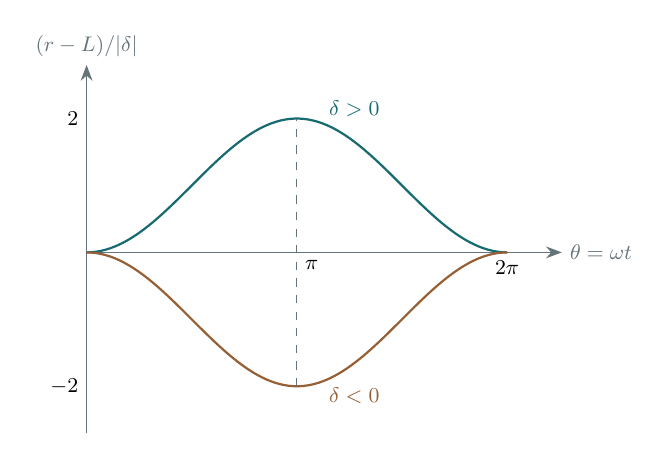
\begin{tikzpicture}[scale=.85,transform shape]

\draw[axis] (0,0)--(7.1,0) node[right] {$\theta=\omega t$};
\draw[axis] (0,-2.7)--(0,2.8) node[above] {$(r-L)/|\delta|$};
\draw[traj,domain=0:6.2832,samples=90] plot (\x,{1-cos(deg(\x))});
\draw[thick,color=warm,domain=0:6.2832,samples=90] plot (\x,{-1+cos(deg(\x))});
\draw[guide] (3.14159,-2)--(3.14159,2);
\node[left] at (0,2) {$2$};\node[left] at (0,-2) {$-2$};
\node[below right] at (3.14159,0) {$\pi$};
\node[below] at (6.2832,0) {$2\pi$};
\node[above,color=accent] at (4,1.9) {$\delta>0$};
\node[below,color=warm] at (4,-1.9) {$\delta<0$};

\end{tikzpicture}
\figcaption{解图电试1.1B\quad 伸长分支超过L，压缩分支的最大值已是初始L。}
\end{minipage}\end{center}
解图电试1.1B分别画$\delta>0$和$\delta<0$的间距变化，二者都从$L$以零斜率出发。
\begin{enumerate}
\item 若$m_1Q_2>m_2Q_1$，球2的自由电加速度较大，弹簧开始伸长。间距在$L$与$L+2\delta$之间变化，故
\[
\boxed{r_{\max}=L+
\frac{2(m_1Q_2-m_2Q_1)E}{k(m_1+m_2)}}.
\]
最大值首次出现在$t=\pi/\omega$。
\item 若$m_1Q_2=m_2Q_1$，两球自由电加速度相等，相对驱动力为零，弹簧始终不伸缩，$r(t)=L$。
\item 若$m_1Q_2<m_2Q_1$，球1的自由电加速度较大，弹簧开始压缩。间距范围为$L+2\delta\le r\le L$，因此初始长度$L$就是间距的最大值。题设的“不相碰”要求$L+2\delta>0$。
\end{enumerate}
合写为
\[
\boxed{r_{\max}=L+\frac{2E}{kM}
\max(m_1Q_2-m_2Q_1,0)}.
\]
\textbf{把相对运动还原为两球的振动。}图C在同一质心坐标中列出初始、平衡和另一转点的位置。令$\xi_i=x_i-X$，则$m_1\xi_1+m_2\xi_2=0$，两球分别位于$-m_2r/M$和$m_1r/M$。在随质心加速而不转动的参考系中，每球增加惯性力$-m_i a_C$，合力为
\[
F_1^{(C)}=Q_1E+k(r-L)-m_1a_C=-F_d+k(r-L),
\qquad F_2^{(C)}=F_d-k(r-L).
\]
由质心约束消去另一球的位置，得到
\[
F_1^{(C)}=-\frac{kM}{m_2}(\xi_1-\xi_{1e}),\quad
F_2^{(C)}=-\frac{kM}{m_1}(\xi_2-\xi_{2e}),
\]
\[
\xi_{1e}=-\frac{m_2}{M}(L+\delta),\qquad
\xi_{2e}=\frac{m_1}{M}(L+\delta).
\]
平衡时两球相对于加速质心保持固定位置，在地面系中仍共同具有$a_C$的加速度，各球所受合力为$m_i a_C$。两式分别除以各自质量，角频率均为$\sqrt{kM/(m_1m_2)}$，与相对坐标方法一致。

初始质心位置取零时，$\xi_1(0)=-m_2L/M$、$\xi_2(0)=m_1L/M$，故各自离平衡点的有向位移为
\[
\xi_1(0)-\xi_{1e}=\frac{m_2}{M}\delta,\qquad
\xi_2(0)-\xi_{2e}=-\frac{m_1}{M}\delta.
\]
两球初始相对速度为零，因而
\[
\xi_1(t)=\xi_{1e}+\frac{m_2\delta}{M}\cos\omega t,\qquad
\xi_2(t)=\xi_{2e}-\frac{m_1\delta}{M}\cos\omega t.
\]
两球同频、反相，质量加权位移和始终为零，初始相位由同一组初值确定。各球振幅为$A_1=m_2|\delta|/M$、$A_2=m_1|\delta|/M$。到$t=\pi/\omega$时，每球走到相反转点，离开初始位置的距离为$2A_i$。若$\delta>0$，两球向外分开，间距增加$2(A_1+A_2)=2\delta$；若$\delta<0$，这组位移使两球靠近，对应最小间距。图C中压缩分支的两个平衡点均在初始位置内侧，伸长分支则均在外侧。

\begin{center}\begin{minipage}{.98\linewidth}\centering
\begin{tikzpicture}[scale=.87,transform shape]
\draw[guide] (0,.6)--(0,-6.1);\node[above]at(0,.6){$C:\ \xi=0$};
\node[anchor=east]at(-2.3,.05){$\delta>0$};\node[anchor=east]at(-2.3,-3.55){$\delta<0$};
\foreach \y/\a/\b/\lab in {0/-1/2/{初始},-1/-1.2/2.4/{平衡},-2/-1.4/2.8/{另一转点},-3.6/-1/2/{初始},-4.6/-.8/1.6/{平衡},-5.6/-.6/1.2/{另一转点}}{
 \draw[axis](-1.8,\y)--(3.35,\y);\node[anchor=east]at(-1.9,\y){\lab};
 \fill[accent](\a,\y)circle(2pt)node[above]{$1$};\fill[warm](\b,\y)circle(2pt)node[above]{$2$};
}
\node[right]at(3.5,0){$r=L$};\node[right]at(3.5,-1){$r=L+\delta$};\node[right]at(3.5,-2){$r=L+2\delta$};
\node[right]at(3.5,-3.6){$r=L$};\node[right]at(3.5,-4.6){$r=L+\delta$};\node[right]at(3.5,-5.6){$r=L+2\delta$};
\node[below]at(.5,-6.15){示例 $m_1:m_2=2:1,\ L=3,\ |\delta|=0.6$，各长度共用同一单位};
\end{tikzpicture}
\figcaption{解图电试1.1C\quad 质量加权的质心位置、平衡位置与同步转点}
\end{minipage}\end{center}

\textbf{能量中的整体项与伸缩项。}图D按相对坐标画出有效势能。由坐标变换直接展开两球动能，可得
\[
T=\frac12M\dot X^2+\frac12\mu\dot r^2,
\qquad Q_1x_1+Q_2x_2=(Q_1+Q_2)X+\frac{m_1Q_2-m_2Q_1}{M}r.
\]
上述坐标恒等式在$E=0$时仍成立，电场所做的功为零。均匀电场对整体坐标的功为$(Q_1+Q_2)E\,\Delta X$，对相对坐标的功为$F_d\Delta r$。相对运动因而满足
\[
\frac12\mu\dot r^2+\frac12k(r-L)^2-F_d(r-L)=0,
\]
初始常数已按$r=L,\dot r=0$取定。配方后，相对运动的有效能量为
\[
\frac12\mu\dot r^2+\frac12k(r-L-\delta)^2
=\frac12k\delta^2.
\]
图D的水平能量线与抛物线交于$r=L$和$r=L+2\delta$。弹簧达到最大形变量时相对动能为零，系统仍保留同一时刻的质心动能。计算两球全部动能时，还须计入电场对质心所做的功。

\begin{center}\begin{minipage}{.98\linewidth}\centering
\begin{tikzpicture}[scale=.86,transform shape]
\draw[axis](-.2,0)--(5.9,0)node[right]{$u=(r-L)/\delta$};
\draw[axis](0,-.2)--(0,3.3)node[above right]{$V_{\rm eff}/(k\delta^2/2)$};
\draw[traj,domain=0:2.15,samples=70]plot({2.5*\x},{2*(\x-1)^2});
\draw[guide](0,2)--(5.45,2)node[right]{$\mathcal H_{\rm rel}=k\delta^2/2$};
\fill[accent](0,2)circle(2pt);\fill[accent](5,2)circle(2pt);
\node[above right]at(0,2){初始 $r=L$};\node[above left]at(5,2){另一转点 $r=L+2\delta$};
\node[below]at(2.5,0){$1$};\node[below]at(5,0){$2$};\node[left]at(0,2){$1$};
\node[below]at(2.5,-.6){图示 $\delta>0$；最低点为 $r_e=L+\delta$};
\end{tikzpicture}
\figcaption{解图电试1.1D\quad 相对有效势能的两个转点，图示 $\delta>0$ 的分支}
\end{minipage}\end{center}

两转点之间的间距范围可统一写成
\[
r_{\min}=L+2\min(\delta,0),\qquad
r_{\max}=L+2\max(\delta,0).
\]
题设要求$r_{\min}>0$。压缩分支只有在$L+2\delta>0$时才允许沿本模型走完整周期；等号已经发生接触。$\delta=0$时所有时刻都保持$r=L$，按恒定间距处理。两球共同加速与内部长度不变可以同时成立。



\Needspace{13\baselineskip}

\pdfbookmark[2]{第 2 题 半无限导线向平面径向分流的磁场}{q2}

\section*{第 2 题\quad 半无限导线向平面径向分流的磁场}\label{q:2}


稳恒电流$I$沿负$x$半轴流向原点$O$，到达$x=0$的无限大平面后均匀向各径向散开。平面上的面电流密度为
\[
\boldsymbol K(\rho)=\frac{I}{2\pi\rho}\hat{\boldsymbol\rho},\qquad \rho>0.
\]
求右半空间$x>0$、左半空间$x<0$以及平面两侧的磁场。规定$\hat{\boldsymbol\phi}$绕$+x$轴按右手方向，真空磁导率为$\mu_0$。另说明理想电流面上以及理想细导线轴线上的场应怎样理解。


\begin{center}\begin{minipage}{.98\linewidth}\centering
\begin{tikzpicture}[scale=.9,transform shape]

\fill[accent!5] (0,-1.7)--(1.8,-.7)--(1.8,2.7)--(0,1.7)--cycle;
\draw[object] (0,-1.7)--(1.8,-.7)--(1.8,2.7)--(0,1.7)--cycle;
\coordinate (O) at (.9,.5);
\draw[object] (-3,.5)--(O);
\draw[motion] (-2.3,.5)--(-.8,.5) node[midway,above] {$I$};
\foreach \ang in {20,80,140,200,260,320}{
\draw[motion] (O)--({.9+.7*cos(\ang)},{.5+1.45*sin(\ang)});}
\draw[axis] (O)--(4,.5) node[right] {$+x$};
\fill (O) circle (1.6pt) node[below right] {$O$};
\node at (.9,3.1) {$x=0$，无限径向分流面};
\node at (1,-2.4) {$K_\rho=I/(2\pi\rho)$};

\end{tikzpicture}
\figcaption{图电试1.2\quad 轴向电流在O转为面内径向电流，构型绕x轴对称。}
\end{minipage}\end{center}

\Needspace{6\baselineskip}\subsection*{解答}


图电试1.2中的电流构型绕$x$轴旋转不变。包含$x$轴的任一平面也是电流的镜面对称面；磁场是轴矢量，其在这个平面内的分量在反射下反号。因而平面内场只能垂直该平面，即
\[
\boldsymbol B=B_\phi(x,\rho)\hat{\boldsymbol\phi}.
\]
在固定$x,\rho$的圆周上，$B_\phi$为常量，可对垂直$x$轴的圆盘用安培环路定律：
\[
2\pi\rho B_\phi=\mu_0I_{\rm through}.
\]
\begin{center}\begin{minipage}{.98\linewidth}\centering
\begin{tikzpicture}[scale=.8,transform shape]

\draw[axis] (-3.3,0)--(3.5,0) node[right] {$x$};
\draw[object] (-3,0)--(0,0);
\draw[motion] (-2.6,0)--(-1.4,0) node[midway,above] {$I$};
\draw[object] (0,-2)--(0,2) node[above] {$x=0$};
\draw[traj] (-2,0) ellipse (.35 and 1.25);
\draw[traj] (2,0) ellipse (.35 and 1.25);
\node[above] at (-2,1.45) {$I_{\rm through}=I$};
\node[above] at (2,1.45) {$I_{\rm through}=0$};
\node[below] at (-2,-1.5) {$B=\mu_0I/(2\pi\rho)$};
\node[below] at (2,-1.5) {$B=0$};
\draw[force] (0,.2)--(0,1.7);\draw[force] (0,-.2)--(0,-1.7);
\node[right] at (.1,-2) {面内电流};

\end{tikzpicture}
\figcaption{解图电试1.2A\quad 圆形环路的方向对称性使安培积分可化为$2\pi\rho B$。}
\end{minipage}\end{center}
解图电试1.2A将两个同半径环路分别放在平面左右。
右侧圆盘没有电流穿过，所以
\[
\boxed{\boldsymbol B(x>0,\rho)=0}.
\]
左侧圆盘被沿$+x$流动的导线电流$I$穿过，故对$\rho>0$
\[
\boxed{\boldsymbol B(x<0,\rho)
=\frac{\mu_0I}{2\pi\rho}\hat{\boldsymbol\phi}}.
\]
右侧轴线上没有导线，磁场也为零。左侧外场公式的适用范围为$\rho>0$；理想线电流所在的轴线是电流分布的奇点，局部场在该模型中未定义。

解图电试1.2B把总场分成半无限导线场与面电流场，显示两分量在平面两侧的相加关系。
\begin{center}\begin{minipage}{.98\linewidth}\centering
\begin{tikzpicture}[scale=.85,transform shape]

\draw[axis] (-3.4,0)--(3.7,0) node[right] {$x/\rho$};
\draw[axis] (0,-1.5)--(0,2.8) node[above] {$4\pi\rho B_\phi/(\mu_0I)$};
\draw[traj,domain=-3:3,samples=90] plot (\x,{1-\x/sqrt(1+\x*\x)});
\draw[thick,color=warm,domain=-3:-.015,samples=65] plot (\x,{1+\x/sqrt(1+\x*\x)});
\draw[thick,color=warm,domain=.015:3,samples=65] plot (\x,{-1+\x/sqrt(1+\x*\x)});
\node[above,color=accent] at (-1.8,2) {半导线};
\node[below,color=warm] at (1.7,-.7) {径向面};
\node[left] at (0,1) {$1$};\node[left] at (0,-1) {$-1$};
\node at (0,-2.1) {右侧相消，左侧相加；面场关于x为奇函数};

\end{tikzpicture}
\figcaption{解图电试1.2B\quad 固定$\rho$处拆分导线与径向面电流的方位场。}
\end{minipage}\end{center}
半无限导线在点$(x,\rho)$产生
\[
B_{\rm wire}
=\frac{\mu_0I}{4\pi}
\int_{-\infty}^0
\frac{\rho\,\mathrm dx'}{[(x-x')^2+\rho^2]^{3/2}}
=\frac{\mu_0I}{4\pi\rho}
\left(1-\frac{x}{\sqrt{x^2+\rho^2}}\right).
\]
这里$B_{\rm wire}$方向取$+\hat{\boldsymbol\phi}$。由总场减去导线场，面电流场为
\[
B_{\rm sheet}=
\begin{cases}
-\dfrac{\mu_0I}{4\pi\rho}
\left(1-\dfrac{x}{\sqrt{x^2+\rho^2}}\right),&x>0,\\[6pt]
\dfrac{\mu_0I}{4\pi\rho}
\left(1+\dfrac{x}{\sqrt{x^2+\rho^2}}\right),&x<0.
\end{cases}
\]
在右侧它恰好抵消导线场；在左侧它与导线场同向，使总场成为完整无限直导线的外部场。面电流场对$x$为奇函数，符合平面对称性。

图B还显示了远场和近面的变化。固定$\rho$而$x\to+\infty$时，导线场与面场都趋零，且始终精确相消；$x\to-\infty$时，半导线场趋向$\mu_0I/(2\pi\rho)$，面场趋零，总场保持同一个无限直导线值。令$x\to0^\pm$，导线场在两侧连续，均为$\mu_0I/(4\pi\rho)$；面场则分别趋于负、正的同一数值。由这三组极限可以逐项读出图C的总场跳变。


\begin{center}\begin{minipage}{.98\linewidth}\centering
\begin{tikzpicture}[scale=.8,transform shape]

\draw[axis] (-3.3,0)--(3.5,0) node[right] {$x$};
\draw[axis] (0,-.6)--(0,2.9) node[above] {$2\pi\rho B_\phi/(\mu_0I)$};
\draw[traj,line width=1.2pt] (-3,2)--(-.05,2);
\draw[traj,line width=1.2pt] (.05,0)--(3,0);
\draw[guide] (0,0)--(0,2);
\draw[accent,fill=white] (0,2) circle (2pt);
\draw[accent,fill=white] (0,0) circle (2pt);
\fill[warm] (0,1) circle (2pt);
\node[left] at (0,2) {$1$};
\node[right] at (.2,1) {主值 $1/2$};
\node at (-1.8,2.7) {$x<0$};
\node at (1.8,.5) {$x>0$};
\node at (0,-1.3) {$\hat x\times(\boldsymbol B_{0^+}-\boldsymbol B_{0^-})=\mu_0\boldsymbol K$};

\end{tikzpicture}
\figcaption{解图电试1.2C\quad 面上场有跃变，标出的中间点是对称主值约定。}
\end{minipage}\end{center}
解图电试1.2C在固定$\rho>0$处画磁场跳变。总场的两个一侧极限为
\[
\boxed{B_\phi(0^-)=\frac{\mu_0I}{2\pi\rho},\qquad
B_\phi(0^+)=0}.
\]
取法线$\hat{\boldsymbol n}=\hat x$，两侧场之差满足
\[
\hat x\times(\boldsymbol B_{0^+}-\boldsymbol B_{0^-})
=\hat x\times\left(-\frac{\mu_0I}{2\pi\rho}\hat\phi\right)
=\mu_0\frac{I}{2\pi\rho}\hat\rho
=\mu_0\boldsymbol K.
\]
这两个单侧值相差$\mu_0I/(2\pi\rho)$；理想零厚度面上的场值由所选取值规则确定。若观察点移到面内$P=(0,\rho,0)$，应采用对称排除观察点小邻域的积分。此时所有面内电流元与位矢的叉乘垂直该面；成对元的法向贡献相消，沿$OP$的电流元与位矢平行，贡献为零。因此面场的对称主值为零，总场主值等于半导线场。面外逼近保留了局部电流片的有限跳变，因此给出图C的两个单侧极限；面内的对称积分给出中间的主值。


若采用对称薄层中面或主值约定，取平均场
\[
\boxed{\boldsymbol B_{\rm pv}(0,\rho)
=\frac12(\boldsymbol B_{0^-}+\boldsymbol B_{0^+})
=\frac{\mu_0I}{4\pi\rho}\hat\phi}.
\]
平均场就是半无限导线在$x=0$的场；面电流的对称主值贡献为零。图C中，平均场为中间的实心点，左右极限分别为上下两个空心点。

\textbf{从成对电流元看面电流的方向。}图D左侧从$+x$方向看分流平面，半径$s$处的电流在两个夹角分别为$\theta,-\theta$的小扇区中向外流。以$y$向右、$z$向上，取观察点$P=(x,\rho,0)$且$\rho>0$。两电流元关于$xy$平面对称，距离$P$相等；把它们各自的电流方向分成$y,z$分量，再分别与从该元指向$P$的位矢作叉乘。这对电流元产生的$x,y$场分量相消，$z$场分量相加。遍历全部成对电流元，面电流场便只沿$\hat\phi$；在选定的$y>0,z=0$半平面，$\hat\phi=\hat z$。图D右侧把其方向与导线场比较，右侧面场沿$-\hat\phi$，左侧沿$+\hat\phi$。

\begin{center}\begin{minipage}{.98\linewidth}\centering
\begin{tikzpicture}[scale=.84,transform shape]

\begin{scope}
\draw[axis](-2.2,0)--(2.4,0)node[right]{$y$};\draw[axis](0,-1.8)--(0,2)node[above]{$z$};
\draw[guide](0,0)circle(1.5);\fill(0,0)circle(1.5pt)node[below left]{$O$};
\foreach \a in{40,-40}{\draw[motion](0,0)--({1.5*cos(\a)},{1.5*sin(\a)});\fill[accent]({1.5*cos(\a)},{1.5*sin(\a)})circle(2pt);}
\draw[guide](1.149,-.964)--(1.149,.964);\node[above right]at(1.149,.964){$(s\cos\theta,s\sin\theta)$};\node[below right]at(1.149,-.964){$(s\cos\theta,-s\sin\theta)$};
\node[below]at(0,-2.3){沿 $+x$ 看电流平面，$P$ 在 $xy$ 平面};
\end{scope}
\begin{scope}[xshift=7cm]
\draw[axis](-2.1,0)--(2.2,0)node[right]{$x$};\draw[object](0,-1.8)--(0,1.8)node[above]{$x=0$};
\node[above]at(-1.2,.9){$B_{\rm sheet}>0$};\node[below]at(1.2,-.9){$B_{\rm sheet}<0$};
\node at(-1.2,.35){$\odot\ \hat\phi$};\node at(1.2,-.35){$\otimes\ -\hat\phi$};
\node[below]at(0,-2.3){固定 $\rho>0$；导线场在两侧均沿 $+\hat\phi$};
\end{scope}

\end{tikzpicture}
\figcaption{解图电试1.2D\quad 电流元成对分解与面场的反向对称}
\end{minipage}\end{center}

把这组成对关系写入毕奥--萨伐尔式，可以逐项得到面场的方向。径向电流面内面积元为$s\,\dd s\,\dd\theta$，由$K=I/(2\pi s)$可知进入积分的电流矢量为
\[
\boldsymbol K\,\dd S=\frac{I}{2\pi}(0,\cos\theta,\sin\theta)\,\dd s\,\dd\theta.
\]
从该元指向$P$的矢量是$\boldsymbol R=(x,\rho-s\cos\theta,-s\sin\theta)$，故叉乘的三个分量正比于
\[
(-\rho\sin\theta,\ x\sin\theta,\ -x\cos\theta).
\]
前两个分量在$\theta$与$-\theta$间相消，第三个分量给出
\[
B_{{\rm sheet},\phi}(x,\rho)
=-\frac{\mu_0Ix}{8\pi^2}
\int_0^\infty\!\dd s\int_0^{2\pi}
\frac{\cos\theta\,\dd\theta}
{(x^2+\rho^2+s^2-2\rho s\cos\theta)^{3/2}}.
\]
对固定$s>0$，将$\cos\theta>0$与其相反角度配对，前者离$P$较近、分母较小，故角积分为正。这个配对比较说明了图D中靠近$P$一侧的贡献为何较大，并确定了面场的符号。分母对$x$为偶函数，式前另有$x$，所以面场对$x$为奇函数；$x>0$时为负，$x<0$时为正。上述积分给出面电流独自产生的场。

轴线上的取值由实际电流分布决定。右半轴$\rho=0,x>0$不含电流，由对称性及两侧连续极限得到零场。负半轴上则有理想线电流，外部$1/\rho$式在趋近轴线时发散；电流中心点还兼有面电流的注入奇点。真实导线中心的场由有限截面内的电流分布及接点结构决定。远离接点的均匀长圆柱导线，可用其截面内的包围电流求内部场；接点附近则按实际弯折与分流结构计算。



\Needspace{13\baselineskip}

\pdfbookmark[2]{第 3 题 水平磁场中下落带电球的临界轨迹}{q3}

\section*{第 3 题\quad 水平磁场中下落带电球的临界轨迹}\label{q:3}


质量$m$、正电荷$q$的小球在离水平地面高度$h$处由静止开始运动，只受重力和匀强磁场的洛伦兹力。磁场水平，空气阻力、辐射忽略，$g$为常量。
求使小球始终不接触地面的磁感应强度条件，给出临界场值及其轨迹，并说明“严格不接触”时是否存在可取得的最小磁场。
取$x$向右、$y$竖直向下，原点为初始位置，磁场沿$\hat x\times\hat y$方向。


\begin{center}\begin{minipage}{.98\linewidth}\centering
\begin{tikzpicture}[scale=.9,transform shape]

\draw[axis] (0,0)--(5,0) node[right] {$x$};
\draw[axis] (0,0)--(0,-3.7) node[below] {$y$};
\draw[object] (-.5,-3)--(5,-3);
\fill[muted!15] (-.5,-3) rectangle (5,-3.2);
\fill[accent] (0,0) circle (2pt) node[above left] {$O:\ m,q$};
\draw[force] (.4,-.1)--(.4,-1) node[right] {$mg$};
\draw[axis,<->] (4.4,0)--(4.4,-3) node[midway,right] {$h$};
\node at (2.6,-.7) {$\otimes\ \boldsymbol B$};
\node at (2.8,-2.6) {地面 $y=h$};

\end{tikzpicture}
\figcaption{图电试1.3\quad 坐标y向下，磁场指向纸内；初始速度为零。}
\end{minipage}\end{center}

\Needspace{6\baselineskip}\subsection*{解答}


图电试1.3中地面为$y=h$，磁场垂直运动平面。记
\[
\omega=\frac{qB}{m}>0.
\]
按题图的右手坐标，$\boldsymbol B=B\hat z$、$\boldsymbol g=g\hat y$，速度始终在$xy$平面内。由叉乘直接得到
\[
q\boldsymbol v\times\boldsymbol B=qB(v_y\hat x-v_x\hat y).
\]
因此向下速度产生向右磁力，向右速度产生向上磁力。初始速度为零时磁力也为零，竖直初加速度为$g$。洛伦兹力分量给
\[
\dot v_x=\omega v_y,\qquad
\dot v_y=g-\omega v_x,\qquad v_x(0)=v_y(0)=0.
\]
选取恒定水平速度，使它的磁力抵消重力，可将含$g$的方程化为纯旋转方程。这给出
\[
q\boldsymbol v_d\times\boldsymbol B=-mg\hat y,
\qquad v_d=\frac{mg}{qB}=\frac g\omega.
\]
把速度分为这项常量漂移和相对速度：
\[
\boldsymbol v=\boldsymbol v_d+\boldsymbol w,\qquad
\boldsymbol v_d=\frac g\omega\hat x.
\]
漂移速度的磁力恰向上抵消重力，故
\[
\dot w_x=\omega w_y,\qquad \dot w_y=-\omega w_x,
\quad
\boldsymbol w(0)=-\frac g\omega\hat x.
\]
\begin{center}\begin{minipage}{.98\linewidth}\centering
\begin{tikzpicture}[scale=.85,transform shape]

\draw[axis] (0,0)--(4,0) node[right] {$v_x$};
\draw[axis] (0,1.9)--(0,-2) node[below] {$v_y$};
\draw[object] (1.5,0) circle (1.5);
\draw[motion] (0,0)--(1.5,0) node[midway,above] {$\boldsymbol v_d$};
\draw[motion] (1.5,0)--(.75,-1.299) node[midway,right] {$\boldsymbol w$};
\draw[force] (0,0)--(.75,-1.299);
\draw[guide] (.375,-.65)--(-.45,-.8);
\node[left] at (-.45,-.8) {$\boldsymbol v$};
\fill (1.5,0) circle (1.5pt) node[above right] {$g/\omega$};
\node at (2.2,2.1) {$|\boldsymbol w|=g/\omega$};
\node[above left] at (0,0) {初态};

\end{tikzpicture}
\figcaption{解图电试1.3A\quad 实际速度是漂移速度与旋转速度相加，速度圆经过零点。}
\end{minipage}\end{center}
在以$\boldsymbol v_d$平移的参考系中，重力与漂移所对应的那部分磁力抵消，剩余合力为$q\boldsymbol w\times\boldsymbol B$。该力随$\boldsymbol w$转向，始终垂直$\boldsymbol w$，因此相对速度的大小保持不变，方向连续旋转。回旋角速度由力与相对速度之比确定，为$qB/m$；相对速度转过一周所需时间为$2\pi/\omega$。这就把恒定重力作用下的运动化成了一个圆心匀速平移、半径保持不变的运动。

解图电试1.3A中的速度圆以$\boldsymbol v_d$为圆心。由旋转方程，
\[
\frac{\dd}{\dd t}(w_x^2+w_y^2)
=2w_x\omega w_y-2w_y\omega w_x=0,
\qquad |\boldsymbol w|=\frac g\omega.
\]
相对速度的初始方向向左，随后转向下方。对$w_x$再求导，得$\ddot w_x+\omega^2w_x=0$；以$w_x(0)=-g/\omega,\dot w_x(0)=0$确定余弦项，并由$w_y=\dot w_x/\omega$求得正弦项。加上向右的$\boldsymbol v_d$，实际速度为：
\[
\boxed{v_x=\frac g\omega(1-\cos\omega t),\qquad
v_y=\frac g\omega\sin\omega t}.
\]
分别对两速度分量积分，水平方向的常量项给$(g/\omega)t$，余弦项给$-(g/\omega^2)\sin\omega t$；竖直方向给$-(g/\omega^2)\cos\omega t$及积分常量$g/\omega^2$。用$x(0)=y(0)=0$得到
\[
\boxed{x=a(\omega t-\sin\omega t),\qquad
y=a(1-\cos\omega t)},\qquad
a=\frac g{\omega^2}=\frac{m^2g}{q^2B^2}.
\]
解图C给出轨迹的几何合成。令$\theta=\omega t$，滚圆圆心为$C=(a\theta,a)$，圆上一点相对圆心的坐标为$(-a\sin\theta,-a\cos\theta)$。圆心以$a\omega=g/\omega$向右平移，半径矢量以角速度$\omega$转动；两个坐标相加正好是上式。圆的半径$a=m v_d/(qB)$同时等于相对回旋半径。初始点位于圆的最高点，相对速度向左与圆心速度相消，满足由静止释放的初态。

\begin{center}\begin{minipage}{.98\linewidth}\centering
\begin{tikzpicture}[scale=.86,transform shape]

\draw[axis](-.5,0)--(5,0)node[right]{$x$};\draw[axis](0,.3)--(0,-2.9)node[below]{$y$};
\draw[object](1.5708,-1)circle(1);\fill[accent](1.5708,-1)circle(2pt)node[right]{$C=(a\theta,a)$};
\fill[warm](.5708,-1)circle(2pt)node[left]{$P$};\draw[guide](1.5708,-1)--(.5708,-1)node[midway,below]{$a$};
\draw[motion](1.5708,-.75)--(3,-.75)node[right]{$v_d=a\omega$};\draw[motion](.5708,-1.15)--(.5708,-1.9)node[below]{$\boldsymbol w$};
\draw[guide](1.5708,-1)--(1.5708,0);\node[above]at(1.5708,0){圆心上方切点};\node[below]at(2.5,-2.6){图示 $\theta=\pi/2$，圆沿顶部水平线滚动};

\end{tikzpicture}
\figcaption{解图电试1.3C\quad 平移圆心与旋转半径共同生成摆线}
\end{minipage}\end{center}
摆线的$y$最大值为$2a$，首次发生在$\omega t=\pi$；该时刻竖直速度为零，水平方向仍有速度$2g/\omega$。
\begin{center}\begin{minipage}{.98\linewidth}\centering
\begin{tikzpicture}[scale=.85,transform shape]

\draw[axis] (0,0)--(7,0) node[right] {$x$};
\draw[axis] (0,0)--(0,-2.9) node[below] {$y$};
\draw[object] (-.3,-2)--(6.8,-2);
\draw[traj,domain=0:6.283185,samples=110] plot ({\x-sin(deg(\x))},{-1+cos(deg(\x))});
\draw[thick,dashed,color=warm,domain=0:6.283185,samples=110] plot ({.75*(\x-sin(deg(\x)))},{-.75*(1-cos(deg(\x)))});
\fill (3.14159,-2) circle (1.6pt) node[below] {临界接触};
\node[above,color=accent] at (5,-.8) {$B=B_*$};
\node[above,color=warm] at (2,-1.2) {$B>B_*$};
\node[right] at (6.8,-2) {$y=h$};
\draw[axis,<->] (6.5,0)--(6.5,-2) node[midway,right] {$h=2a_*$};
\node[below] at (0,0) {$O$};

\end{tikzpicture}
\figcaption{解图电试1.3B\quad 临界摆线相切地面；更强磁场的虚线轨迹仍留间隙。}
\end{minipage}\end{center}
沿图B的第一段轨迹观察，$0<\theta<\pi$时$\sin\theta>0$，所以竖直速度向下；$\pi<\theta<2\pi$时竖直速度向上。四分之一周期时，$x=a(\pi/2-1),y=a$，两速度分量同为$g/\omega$，切线向右下方；半周期时下落到$2a$，切线转为水平。后半周期回升到初始高度，水平方向仍在前进，于是相邻两个零速度尖点之间构成一个完整摆线拱。

固定$m,q,g$而增强磁场，时间尺度$1/\omega$按$1/B$减小，空间尺度$a$按$1/B^2$减小，速度尺度$g/\omega$按$1/B$减小。因而小球更早转入上升段，最大下落量也更小。图B中虚线摆线的高度和每个拱的水平宽度同时缩小，地面位置则由给定的$h$保持不变。判定场强时，正是比较这个随场变化的最大下落量与固定地面高度。

解图电试1.3B把地面画在初始水平线下$h$处。严格不接触要求摆线最低点仍在地面上方，即
\[
2a<h
\quad\Longleftrightarrow\quad
\boxed{B>B_*},\qquad
\boxed{B_*=\frac m q\sqrt{\frac{2g}{h}}}.
\]
在$B=B_*$时，$a=h/2$，临界轨迹为
\[
x=\frac h2(\theta-\sin\theta),\qquad
y=\frac h2(1-\cos\theta),\qquad
\theta=\sqrt{\frac{2g}{h}}\,t.
\]
它在$\theta=(2k+1)\pi$处与地面相切。严格不接触的允许区间是$(B_*,\infty)$，下确界为$B_*$，这个开区间没有可取得的最小场强。等号$B=B_*$描述恰好相切的临界轨迹。

若$0<B<B_*$，第一段下降过程便有$y=h$。由
\[
\cos\theta_c=1-\frac h a,\qquad 0<\theta_c<\pi
\]
可知首次到达地面时小球仍有向下速度，摆线描述从释放到首次接触的这一段运动。具体地，首次接触时刻和水平位置为
\[
t_c=\frac{\theta_c}{\omega},\qquad
x_c=a(\theta_c-\sin\theta_c).
\]
用接触条件$1-\cos\theta_c=h/a$代入速度式，可直接得到
\[
v_{x,c}=\omega h,\qquad
v_{y,c}=\sqrt{2gh-\omega^2h^2}>0.
\]
这两个分量给出到达地面时的方向：场越接近临界值，竖直分量越小、切线越接近水平；在临界等号处，竖直分量为零而水平分量达到$\sqrt{2gh}$。当$B$趋于零，接触时间趋于$\sqrt{2h/g}$，水平分量趋零，竖直分量趋于$\sqrt{2gh}$，连续接到自由落体。$B=0$时直接由$y=gt^2/2$描述下落。

\textbf{最低点的受力与动能变化。}在$\theta=\pi$，$v_y=0$、$v_x=2g/\omega$，向上磁力为$qB(2g/\omega)=2mg$，重力向下为$mg$，所以净加速度向上为$g$。图D的速度箭头水平向右，合力箭头向上，随后小球进入上升段。这个转折由竖直速度的变号确定。

\begin{center}\begin{minipage}{.98\linewidth}\centering
\begin{tikzpicture}[scale=.86,transform shape]

\draw[axis](-1,0)--(4,0)node[right]{$x$};\fill[accent](0,0)circle(3pt)node[below left]{最低点};
\draw[motion](0,.2)--(2.8,.2)node[right]{$v_x=2g/\omega$};
\draw[force](0,.35)--(0,2.35)node[above]{$F_B=2mg$};\draw[force](.3,-.15)--(.3,-1.15)node[below]{$mg$};
\draw[motion](2,-.4)--(2,.6)node[right]{$\boldsymbol a=-g\hat y$};\node[below]at(1.3,-1.9){竖直速度为零时，向上的合力使轨迹转弯};

\end{tikzpicture}
\figcaption{解图电试1.3D\quad 最低点的速度、磁力与重力}
\end{minipage}\end{center}
沿运动方程与速度作点积，磁力项为零，得$m\boldsymbol v\cdot\dot{\boldsymbol v}=mgv_y$。从初态积分即有$mv^2/2=mgy$。把速度分量写入这个能量关系：
\[
v^2=\frac{g^2}{\omega^2}
[(1-\cos\theta)^2+\sin^2\theta]
=2ga(1-\cos\theta)=2gy.
\]
每到$\theta=2k\pi$，位置回到初始高度、速度也再次为零，形成摆线尖点。每个周期水平方向前进$2\pi a$；相对回旋速度恒定，而地面系速率随重力做功周期变化。


\Needspace{13\baselineskip}

\pdfbookmark[2]{第 4 题 弱磁场中异号带电双体的质心摆线}{q4}

\section*{第 4 题\quad 弱磁场中异号带电双体的质心摆线}\label{q:4}


质量均为$m$、电荷分别为$+q$与$-q$的两质点相距$2R$。以其质心$C$为原点，取$x$向右、$y$向上。$t=0$时$+q$在$(0,-R)$、$-q$在$(0,R)$，两者速度构成绕$C$顺时针的半径$R$圆运动，质心初速为零。初始圆运动角频率$\omega$由库仑引力确定。
考察这一初态在沿$+z$的弱匀强静磁场$\boldsymbol B=B\hat z$中的后续运动；忽略重力、辐射及建场过程的感应冲量。取$qB/(m\omega)\ll1$，只求关于$B$的一阶质心运动，近似保持内部圆运动不变。
\begin{enumerate}
\item 求$v_{Cx}(t),v_{Cy}(t)$。
\item 求$X_C(t),Y_C(t)$并画轨迹。
\item 说明这一近似为何不与磁力不做功、系统能量守恒矛盾。
\end{enumerate}


\begin{center}\begin{minipage}{.98\linewidth}\centering
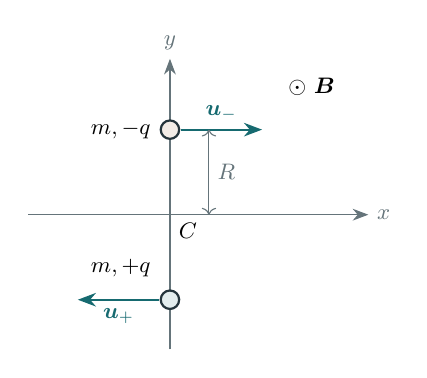
\begin{tikzpicture}[scale=.9,transform shape]

\draw[axis] (-2,0)--(2.8,0) node[right] {$x$};
\draw[axis] (0,-1.9)--(0,2.2) node[above] {$y$};
\fill[accent!12] (0,-1.2) circle (.13);\draw[object] (0,-1.2) circle (.13);
\fill[warm!12] (0,1.2) circle (.13);\draw[object] (0,1.2) circle (.13);
\node[left] at (-.15,1.2) {$m,-q$};\node[above left] at (-.15,-1) {$m,+q$};
\draw[motion] (.15,1.2)--(1.3,1.2) node[midway,above] {$\boldsymbol u_-$};
\draw[motion] (-.15,-1.2)--(-1.3,-1.2) node[midway,below] {$\boldsymbol u_+$};
\node[below right] at (0,0) {$C$};
\node at (2,1.8) {$\odot\ \boldsymbol B$};
\draw[axis,<->] (.55,0)--(.55,1.2) node[midway,right] {$R$};

\end{tikzpicture}
\figcaption{图电试1.4\quad 上方负电荷向右、下方正电荷向左，初始内部运动顺时针。}
\end{minipage}\end{center}

\Needspace{6\baselineskip}\subsection*{解答}


图电试1.4中$+q$在下方，顺时针运动使它的初速度向左。未受磁场扰动的库仑圆运动满足
\[
m\omega^2R=\frac{q^2}{4\pi\varepsilon_0(2R)^2},
\qquad
\boxed{\omega=\frac{q}{4R\sqrt{\pi\varepsilon_0mR}}}.
\]
以零阶内部圆运动作为一阶磁力计算中的速度，
\[
\boldsymbol r_+=(-R\sin\omega t,-R\cos\omega t),\qquad
\boldsymbol r_-=-\boldsymbol r_+,
\]
\[
\boldsymbol u_+=(-\omega R\cos\omega t,\ \omega R\sin\omega t),
\qquad \boldsymbol u_-=-\boldsymbol u_+.
\]
两个粒子的地面速度分别为$\boldsymbol V_C+\boldsymbol u_+$和$\boldsymbol V_C-\boldsymbol u_+$。它们的磁力之和为
\[
\boldsymbol F_{\rm ext}
=q(\boldsymbol V_C+\boldsymbol u_+)\times\boldsymbol B
-q(\boldsymbol V_C-\boldsymbol u_+)\times\boldsymbol B
=2q\boldsymbol u_+\times\boldsymbol B.
\]
质心速度所致的两项在总力中严格相消，内部库仑力也相消。
\begin{center}\begin{minipage}{.98\linewidth}\centering
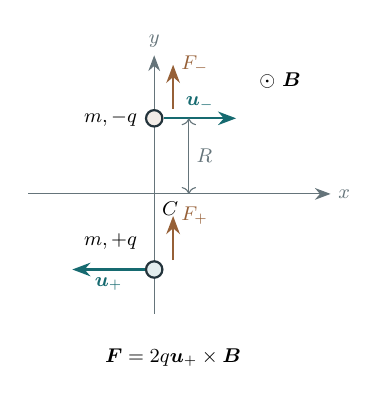
\begin{tikzpicture}[scale=.8,transform shape]

\draw[axis] (-2,0)--(2.8,0) node[right] {$x$};
\draw[axis] (0,-1.9)--(0,2.2) node[above] {$y$};
\fill[accent!12] (0,-1.2) circle (.13);\draw[object] (0,-1.2) circle (.13);
\fill[warm!12] (0,1.2) circle (.13);\draw[object] (0,1.2) circle (.13);
\node[left] at (-.15,1.2) {$m,-q$};\node[above left] at (-.15,-1) {$m,+q$};
\draw[motion] (.15,1.2)--(1.3,1.2) node[midway,above] {$\boldsymbol u_-$};
\draw[motion] (-.15,-1.2)--(-1.3,-1.2) node[midway,below] {$\boldsymbol u_+$};
\node[below right] at (0,0) {$C$};
\node at (2,1.8) {$\odot\ \boldsymbol B$};
\draw[axis,<->] (.55,0)--(.55,1.2) node[midway,right] {$R$};

\draw[force] (.3,1.35)--(.3,2.05) node[right] {$F_-$};
\draw[force] (.3,-1.05)--(.3,-.35) node[right] {$F_+$};
\node at (.3,-2.6) {$\boldsymbol F=2q\boldsymbol u_+\times\boldsymbol B$};

\end{tikzpicture}
\figcaption{解图电试1.4A\quad 异号电荷的内部速度反向，两磁力却同向，初始总力向上。}
\end{minipage}\end{center}
解图电试1.4A中$t=0$两磁力均向$+y$。任意时刻总力分量为
\[
F_x=2q\omega RB\sin\omega t,\qquad
F_y=2q\omega RB\cos\omega t.
\]
总质量为$2m$，故$\dot v_{Cx}=(q\omega RB/m)\sin\omega t$、$\dot v_{Cy}=(q\omega RB/m)\cos\omega t$。从0到$t$积分时，正弦项给$(1-\cos\omega t)/\omega$，余弦项给$\sin\omega t/\omega$。取$\boldsymbol V_C(0)=0$，得
\[
\boxed{v_{Cx}=\frac{qBR}{m}(1-\cos\omega t),\qquad
v_{Cy}=\frac{qBR}{m}\sin\omega t}.
\]
水平方向速度含常量$qBR/m$及余弦项，竖直方向速度为正弦项。分别积分，前者产生匀速平移和正弦位移，后者产生余弦位移。再用$X_C(0)=Y_C(0)=0$确定常数，得到
\[
\boxed{X_C=A(\omega t-\sin\omega t),\qquad
Y_C=A(1-\cos\omega t)},\qquad
A=\frac{qBR}{m\omega}.
\]
代入$\omega$可写
\[
A=4BR^2\sqrt{\frac{\pi\varepsilon_0R}{m}}.
\]
\begin{center}\begin{minipage}{.98\linewidth}\centering
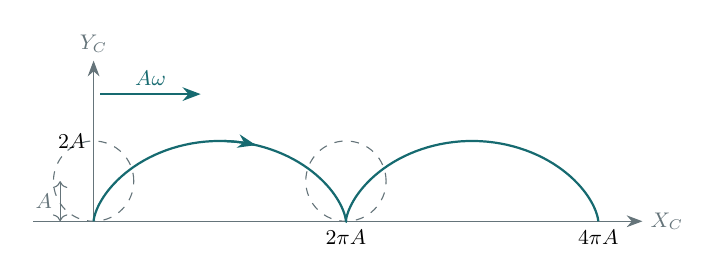
\begin{tikzpicture}[scale=.85,transform shape]

\draw[axis] (-.9,0)--(8.2,0) node[right] {$X_C$};
\draw[axis] (0,0)--(0,2.4) node[above] {$Y_C$};
\draw[guide] (0,.6) circle (.6);
\draw[guide] (3.76991,.6) circle (.6);
\draw[traj,domain=0:12.56637,samples=150] plot ({.6*(\x-sin(deg(\x)))},{.6*(1-cos(deg(\x)))});
\draw[motion,domain=3.2:3.6,samples=20] plot ({.6*(\x-sin(deg(\x)))},{.6*(1-cos(deg(\x)))});
\draw[motion] (.1,1.9)--(1.6,1.9) node[midway,above] {$A\omega$};
\draw[axis,<->] (-.5,0)--(-.5,.6) node[midway,left] {$A$};
\node[below] at (3.76991,0) {$2\pi A$};\node[below] at (7.53982,0) {$4\pi A$};
\node[left] at (0,1.2) {$2A$};

\end{tikzpicture}
\figcaption{解图电试1.4B\quad 漂移与等半径圆运动叠加，质心摆线由零速尖点出发。}
\end{minipage}\end{center}
图B中的两部分位移可具体写成
\[
X_1=-A\sin\omega t,\quad Y_1=A(1-\cos\omega t),\qquad
X_2=A\omega t,\quad Y_2=0.
\]
第一部分满足$X_1^2+(Y_1-A)^2=A^2$，在以$(0,A)$为圆心的圆上顺时针运动；第二部分使圆心向右平移。初始点位于圆的最低处，圆周速度向左，与向右平移速度等大反向，合速度为零。解图电试1.4B把这两部分叠加，得到由零速尖点出发的轨迹。两者速度尺度均为$A\omega=qBR/m$，相位使初始速度恰好相消，故质心轨迹为滚圆半径$A$的摆线。每周期前进$2\pi A$，最大高度$2A$，每到周期末速度降到零，出现尖点。

第（3）问按弱场小参数$\epsilon=qB/(m\omega)\ll1$比较运动与能量。由$A=\epsilon R$，质心位移和速度从一阶出现。具体地，
\[
V_C^2=(A\omega)^2[(1-\cos\omega t)^2+\sin^2\omega t]
=2(A\omega)^2(1-\cos\omega t),
\]
所以质心速率最大$2\epsilon\omega R$。因而质心动能的最大量为
\[
K_{C,\max}=\frac12(2m)(2\epsilon\omega R)^2
=4m\epsilon^2\omega^2R^2,
\]
仅是内部初始总动能$m\omega^2R^2$的$O(\epsilon^2)$。
\begin{center}\begin{minipage}{.98\linewidth}\centering
\begin{tikzpicture}[scale=.8,transform shape]

\draw[object] (0,0) circle (1.4);
\draw[axis] (0,0)--(1.4,0) node[midway,below] {$R$};
\fill (0,0) circle (1.3pt);
\node[above] at (0,1.7) {内部相对轨道};
\draw[object] (4.5,0) circle (.2);
\draw[axis] (4.5,0)--(4.5,.2);
\draw[guide] (4.5,.2)--(5.1,.8);
\node[right] at (5.1,.8) {$A=\epsilon R$};
\node[below] at (4.5,-.6) {质心分解圆};
\node at (2.8,-2) {$K_C/K_{\rm internal}=O(\epsilon^2)$};
\node at (3.3,2.7) {$\epsilon=qB/(m\omega)\ll1$};

\end{tikzpicture}
\figcaption{解图电试1.4C\quad 一阶质心位移与二阶动能分开计量，内部反馈从二阶进入。}
\end{minipage}\end{center}
解图电试1.4C分别标出一阶位移与二阶能量尺度。把两粒子的磁力作差，内部相对方程中的新增项正比于
\[
\frac qm\boldsymbol V_C\times\boldsymbol B=O(B^2).
\]
关于$B$的一阶质心运动可由零阶内部圆运动求出；质心的动能从二阶出现，相同阶次的内部运动变化随之进入机械能分配。

本题在$\epsilon\ll1$、考察有限个内部周期时采用上述一阶质心轨迹。时间尺度延长后，内部相位的高阶变化应通过相对运动方程继续求出。
\textbf{质心与内部能量怎样联系。}令正电荷相对质心的位置为$\boldsymbol r$，其速度为$\boldsymbol u=\dot{\boldsymbol r}$。两粒子的位置为$\boldsymbol C\pm\boldsymbol r$，两条牛顿方程相加给出质心运动，相减给出内部运动：
\[
m\dot{\boldsymbol V}_C=q\boldsymbol u\times\boldsymbol B,
\qquad
m\ddot{\boldsymbol r}=-\frac{q^2}{16\pi\varepsilon_0|\boldsymbol r|^3}\boldsymbol r
+q\boldsymbol V_C\times\boldsymbol B.
\]
第一式就是前面总质量为$2m$的质心方程；第二式显示内部的磁力反馈通过质心速度进入。将第一式从初态积分，还得到静磁场中的精确关系
\[
m\boldsymbol V_C=q[\boldsymbol r(t)-\boldsymbol r(0)]\times\boldsymbol B.
\]
取其零阶内部圆运动，分量立刻给出已求得的$v_{Cx},v_{Cy}$，且$\boldsymbol r$每转一周回到初位时质心速度也回到零。

以$\boldsymbol r/R=\boldsymbol\rho$、$\tau=\omega t$表示内部方程，并用$\boldsymbol\rho_0=(0,-1)$，可化为
\[
\boldsymbol\rho''=-\frac{\boldsymbol\rho}{|\boldsymbol\rho|^3}
-\epsilon^2(\boldsymbol\rho-\boldsymbol\rho_0).
\]
在固定的有限时间区间内，零阶圆轨道的 $|\boldsymbol\rho|=1$，小 $\epsilon$ 时相对方程在其附近光滑，系数 $\epsilon^2$ 使内部位移的改变为 $O(\epsilon^2 R)$。用前面的精确质心速度关系，这一改变在 $V_C/(\omega R)$ 中还要乘 $\epsilon$，所以图B的一阶速度与实际速度相差 $O(\epsilon^3\omega R)$。图C的二阶能量尺度也可直接从这个精确关系读出：
\[
K_C=mV_C^2=\frac{q^2B^2}{m}\big|\boldsymbol r(t)-\boldsymbol r(0)\big|^2.
\]
质心动能对应内部轨迹上从初始位置量起的弦长平方。

系统的质心动能和内部机械能分别为
\[
K_C=mV_C^2,\qquad
E_{\rm int}=m u^2-\frac{q^2}{8\pi\varepsilon_0|\boldsymbol r|}.
\]
沿两条运动方程与各自速度作点积，得到
\[
\dot K_C=2q\boldsymbol V_C\cdot(\boldsymbol u\times\boldsymbol B),
\qquad
\dot E_{\rm int}=2q\boldsymbol u\cdot(\boldsymbol V_C\times\boldsymbol B)
=-\dot K_C.
\]
三重积的反对称性使两项逐时抵消，总机械能$K_C+E_{\rm int}$保持初值。图D用首个非零阶画出这两项的相反变化：质心动能在半周期最大，内部机械能相应减少；周期末质心速度恢复为零，该阶能量也回到内部。每个粒子的磁力始终垂直其完整地面速度，外磁力对系统所做的总功为零。这里分开计算整体运动和内部运动的功率，便能看清两种机械能之间的交换。

\begin{center}\begin{minipage}{.98\linewidth}\centering
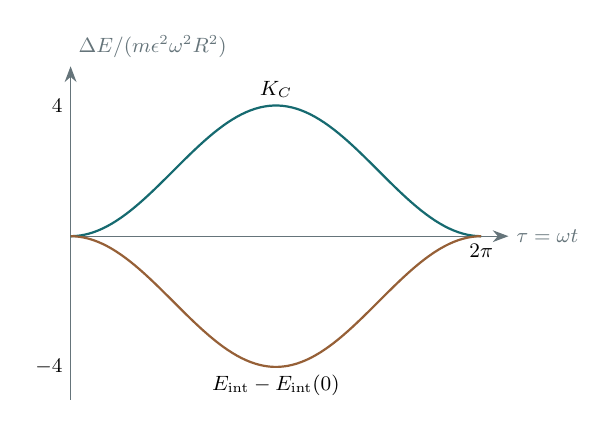
\begin{tikzpicture}[scale=.83,transform shape]

\draw[axis](0,0)--(6.7,0)node[right]{$\tau=\omega t$};\draw[axis](0,-2.5)--(0,2.6)node[above right]{$\Delta E/(m\epsilon^2\omega^2R^2)$};
\draw[traj,domain=0:2*pi,samples=90]plot(\x,{1-cos(deg(\x))});
\draw[thick,color=warm,domain=0:2*pi,samples=90]plot(\x,{-1+cos(deg(\x))});
\node[left]at(0,2){$4$};\node[left]at(0,-2){$-4$};\node[above]at(pi,2){$K_C$};\node[below]at(pi,-2){$E_{\rm int}-E_{\rm int}(0)$};\node[below]at(2*pi,0){$2\pi$};


\end{tikzpicture}
\figcaption{解图电试1.4D\quad 二阶质心动能与内部机械能的相反变化}
\end{minipage}\end{center}



\Needspace{13\baselineskip}

\pdfbookmark[2]{第 5 题 带电容滑动双棒的充电与最终速度}{q5}

\section*{第 5 题\quad 带电容滑动双棒的充电与最终速度}\label{q:5}


两条水平、足够长的平行导轨上有左右两根可无摩擦滑动的导体棒。每根棒长度$l$、质量$m$、电阻$R$，棒中各串接一个电容为$C$的相同电容器，两个电容器初始均未充电；导轨电阻可忽略，组成矩形回路。均匀静磁场$B$垂直回路平面向内。初始左棒静止，右棒以$v_0>0$沿导轨向右运动，初始棒间距$d_0$有限，所有辐射与回路自感忽略。
\begin{enumerate}
\item 对电容$C$的充电过程，能否用静止回路等效：保持两棒的电阻$R$及两电容$C$，再串联一个电容$C'$与恒定电源$\mathcal E'$，于$t=0$闭合？若能，求$\mathcal E',C'$。
\item 求两棒速度、电容电荷随时间的关系。
\item 求两棒最终速度，说明是否相等；带电容时棒间距是否趋向有限值？
\item 将两个电容器取去、用导线接通相应断点，求此时最终速度和棒间距的极限。
\end{enumerate}


\begin{center}\begin{minipage}{.98\linewidth}\centering
\begin{tikzpicture}[scale=.9,transform shape]

\draw[object] (-.6,0)--(5,0);\draw[object] (-.6,2.7)--(5,2.7);
\foreach \x in {0,4}{
\draw[object] (\x,0)--(\x,.95);
\draw[object,line width=1pt] (\x-.36,.95)--(\x+.36,.95);
\draw[object,line width=1pt] (\x-.36,1.15)--(\x+.36,1.15);
\draw[object] (\x,1.15)--(\x,1.8);
\draw[object] (\x-.14,1.8) rectangle (\x+.14,2.35);
\draw[object] (\x,2.35)--(\x,2.7);
\node[right] at (\x+.5,1.05) {$C$};
\node[right] at (\x+.2,2.08) {$R$};
}
\node at (2,1.6) {$\otimes\ B$};
\draw[axis,<->] (-.9,0)--(-.9,2.7) node[midway,left] {$l$};
\draw[motion] (4.15,3.2)--(5.4,3.2) node[midway,above] {$v_0$};
\node[above] at (0,3) {初始静止};
\draw[axis,<->] (0,-.5)--(4,-.5) node[midway,below] {$d_0$};

\end{tikzpicture}
\figcaption{图电试1.5\quad 两棒各串一个C、各有电阻R；初始电容均不带电。}
\end{minipage}\end{center}

\Needspace{6\baselineskip}\subsection*{解答}


图电试1.5规定两棒速度向右为正，记右棒$v_r$、左棒$v_l$；回路电流$I$取逆时针为正。右棒向右时，棒内正电荷所受$\boldsymbol v\times\boldsymbol B$向上，沿逆时针产生正电动势；左棒后来也向右运动，在同一绕行方向中产生相反的电动势。两项相减，使驱动取决于两棒的相对速度。按此方向定义电容电荷$Q(t)=\int_0^t I(t')\,\mathrm dt'$，两个相同电容串联，电压降之和为$2Q/C$。
相对运动产生的总电动势与回路方程为
\[
\mathcal E=Bl(v_r-v_l),\qquad
\boxed{Bl(v_r-v_l)=\frac{2Q}{C}+2RI},\qquad I=\dot Q.
\]
图A中右棒电流向上，安培力向左；左棒电流向下，安培力向右。两力大小相等，水平总动量保持不变。以逆时针电流$I$为同一个累计量，两棒动力学为
\[
m\dot v_r=-BlI,\qquad m\dot v_l=+BlI.
\]
\begin{center}\begin{minipage}{.98\linewidth}\centering
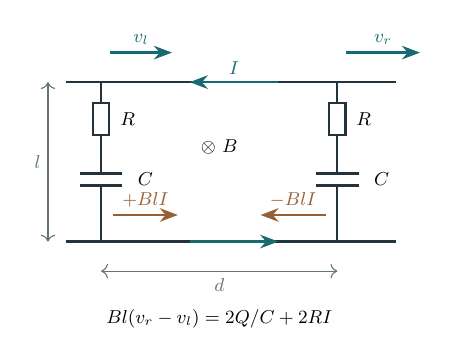
\begin{tikzpicture}[scale=.75,transform shape]

\draw[object] (-.6,0)--(5,0);\draw[object] (-.6,2.7)--(5,2.7);
\foreach \x in {0,4}{
\draw[object] (\x,0)--(\x,.95);
\draw[object,line width=1pt] (\x-.36,.95)--(\x+.36,.95);
\draw[object,line width=1pt] (\x-.36,1.15)--(\x+.36,1.15);
\draw[object] (\x,1.15)--(\x,1.8);
\draw[object] (\x-.14,1.8) rectangle (\x+.14,2.35);
\draw[object] (\x,2.35)--(\x,2.7);
\node[right] at (\x+.5,1.05) {$C$};
\node[right] at (\x+.2,2.08) {$R$};
}
\node at (2,1.6) {$\otimes\ B$};
\draw[axis,<->] (-.9,0)--(-.9,2.7) node[midway,left] {$l$};
\draw[motion] (4.15,3.2)--(5.4,3.2) node[midway,above] {$v_r$};
\draw[motion] (.15,3.2)--(1.2,3.2) node[midway,above] {$v_l$};
\draw[axis,<->] (0,-.5)--(4,-.5) node[midway,below] {$d$};

\draw[force] (3.8,.45)--(2.7,.45) node[midway,above] {$-BlI$};
\draw[force] (.2,.45)--(1.3,.45) node[midway,above] {$+BlI$};
\draw[motion] (3,2.7)--(1.5,2.7) node[midway,above] {$I$};
\draw[motion] (1.5,0)--(3,0);
\node at (2,-1.3) {$Bl(v_r-v_l)=2Q/C+2RI$};

\end{tikzpicture}
\figcaption{解图电试1.5A\quad 逆时针电流使右棒受阻、左棒加速，总水平力相消。}
\end{minipage}\end{center}
解图电试1.5A把这两个安培力与电流标在同一回路。将$I\,\dd t$写为$\dd Q$，从$Q=0$积分到当前电量：右棒的动量改变量为$-BlQ$，左棒为$+BlQ$。两棒初始动量分别为$mv_0$与0，故
\[
\boxed{v_r=v_0-\frac{Bl}{m}Q,\qquad
v_l=\frac{Bl}{m}Q}.
\]
两速度之和始终为$v_0$，质心速度因此保持$v_0/2$。
将其代入回路方程，得到
\[
\boxed{2R\dot Q+
2\left(\frac1C+\frac{B^2l^2}{m}\right)Q=Blv_0}.
\]
这个附加项来自两棒速度差的减小：每累计电量$\dd Q$，右棒速度减小$(Bl/m)\dd Q$，左棒速度增加同样大小，两者使电动势总共减少$(2B^2l^2/m)\dd Q$。电容充电增大$2Q/C$，机械运动使驱动减小；将它与电容电压放在方程同一侧，得到总的电荷系数。

第（1）问的静止回路含三个串联电容，等效串联电容$C_\Sigma$满足
\[
\frac1{C_\Sigma}=\frac2C+\frac1{C'}.
\]
\begin{center}\begin{minipage}{.98\linewidth}\centering
\begin{tikzpicture}[scale=.85,transform shape]

\draw[object] (0,0)--(0,.9);
\draw[object,line width=1pt] (-.35,.9)--(.35,.9);
\draw[object,line width=1pt] (-.35,1.1)--(.35,1.1);
\draw[object] (0,1.1)--(0,1.7);
\draw[object] (-.14,1.7) rectangle (.14,2.25);
\draw[object] (0,2.25)--(0,2.6)--(1.8,2.6);
\draw[object,line width=1pt] (1.8,2.25)--(1.8,2.95);
\draw[object,line width=1pt] (2,2.25)--(2,2.95);
\draw[object] (2,2.6)--(4,2.6)--(4,2.25);
\draw[object] (3.86,1.7) rectangle (4.14,2.25);
\draw[object] (4,1.7)--(4,1.1);
\draw[object,line width=1pt] (3.65,1.1)--(4.35,1.1);
\draw[object,line width=1pt] (3.65,.9)--(4.35,.9);
\draw[object] (4,.9)--(4,0)--(2.1,0);
\draw[object] (2.1,-.35)--(2.1,.35);
\draw[object] (1.9,-.18)--(1.9,.18);
\draw[object] (1.9,0)--(0,0);
\node[above] at (1.9,3) {$C'$};
\node[left] at (-.4,1) {$C$};\node[right] at (4.4,1) {$C$};
\node[left] at (-.2,2) {$R$};\node[right] at (4.2,2) {$R$};
\node[below] at (2,-.5) {$\mathcal E'=Blv_0$};
\node at (2,-1.2) {三个电容串联；初始均未充电};

\end{tikzpicture}
\figcaption{解图电试1.5B\quad 静止等效回路用附加串联电容表示机械反馈。}
\end{minipage}\end{center}
解图电试1.5B中所有电容初始不带电，回路电流经过两个电阻，总电阻仍为$2R$，充电方程为
\[
2R\dot Q+\left(\frac2C+\frac1{C'}\right)Q=\mathcal E'.
\]
逐项比较同一个$Q(t)$所满足的方程，得到
\[
\boxed{\mathcal E'=Blv_0,\qquad
C'=\frac{m}{2B^2l^2}}.
\]
两个回路有相同的总电阻、相同的初始电量和相同的充电微分方程，因此每个时刻的$Q(t)$与$I(t)$相同。新增串联电容的电压$Q/C'=2B^2l^2Q/m$恰好对应机械反馈项。静止回路的能量由恒定电源供给，运动回路的能量由两棒动能供给，分别按各自供能过程计算。

第（2）问记无量纲耦合与时间尺度
\[
\eta=\frac{CB^2l^2}{m},\qquad
\tau=\frac{CR}{1+\eta},\qquad
Q_\infty=\frac{CBlv_0}{2(1+\eta)}.
\]
由$2RC_\Sigma=\tau$，充电方程化为$\dot Q+Q/\tau=Q_\infty/\tau$。乘积分因子$e^{t/\tau}$，
\[
\frac{\dd}{\dd t}(Qe^{t/\tau})=\frac{Q_\infty}{\tau}e^{t/\tau},\qquad
Q(t)e^{t/\tau}-Q(0)=Q_\infty(e^{t/\tau}-1).
\]
取$Q(0)=0$并求导，得到
\[
\boxed{Q(t)=Q_\infty(1-e^{-t/\tau}),\qquad
I(t)=\frac{Blv_0}{2R}e^{-t/\tau}}.
\]
在两棒速度与电量的关系中代入这条充电曲线。右棒减去累计安培冲量对应的速度，左棒增加同样大小；系数$(Bl/m)Q_\infty$化为$v_0\eta/[2(1+\eta)]$。于是
\[
\boxed{v_r(t)=v_0\left[1-\frac{\eta}{2(1+\eta)}(1-e^{-t/\tau})\right]},
\]
\[
\boxed{v_l(t)=v_0\frac{\eta}{2(1+\eta)}(1-e^{-t/\tau})}.
\]
\begin{center}\begin{minipage}{.98\linewidth}\centering
\begin{tikzpicture}[scale=.85,transform shape]

\draw[axis] (0,0)--(5.5,0) node[right] {$t/\tau$};
\draw[axis] (0,0)--(0,3.9) node[above] {$v/v_0$};
\draw[traj,domain=0:4.5,samples=70] plot (\x,{3.5*(.75+.25*exp(-\x))});
\draw[thick,color=warm,domain=0:4.5,samples=70] plot (\x,{3.5*.25*(1-exp(-\x))});
\draw[guide] (0,2.625)--(4.9,2.625);
\draw[guide] (0,.875)--(4.9,.875);
\node[left] at (0,3.5) {$1$};
\node[left] at (0,2.625) {$3/4$};\node[left] at (0,.875) {$1/4$};
\node[above,color=accent] at (2.5,2.9) {$v_r$};
\node[below,color=warm] at (2.5,.6) {$v_l$};
\node at (2.9,3.9) {示例 $\eta=CB^2l^2/m=1$};

\end{tikzpicture}
\figcaption{解图电试1.5C\quad 带电容时充电结束，两棒速度平台仍有间隔。}
\end{minipage}\end{center}
解图电试1.5C中右棒减速、左棒加速，两者最终有不同平台值：
\[
\boxed{v_{r,\infty}=\frac{2+\eta}{2(1+\eta)}v_0,\qquad
v_{l,\infty}=\frac{\eta}{2(1+\eta)}v_0}.
\]
两棒最终相对速度
\[
w_\infty=v_{r,\infty}-v_{l,\infty}=\frac{v_0}{1+\eta}>0.
\]
充电后期，电阻电压$2RI$趋零，剩余的非零运动电动势由两个电容电压共同抵消，即
\[
Blw_\infty=\frac{2Q_\infty}{C}.
\]
电容电压已经抵消非零的运动电动势，故电流停止、两棒却仍以不同速度运动。相对速度全过程为
\[
w(t)=\frac{v_0}{1+\eta}(1+\eta e^{-t/\tau}),
\]
所以棒间距为
\[
\boxed{d(t)=d_0+\frac{v_0}{1+\eta}
\left[t+\eta\tau(1-e^{-t/\tau})\right]}.
\]
对有限$C>0$，相对速度有正的平台$v_0/(1+\eta)$，其时间积分持续增长，间距渐近线性增大。瞬态指数项只提供有限的附加距离$v_0\eta\tau/(1+\eta)$。因此两棒速度各自趋于有限值，同时棒间距趋于无穷大，这两种极限分别由速度本身和速度的时间积分决定。

第（4）问去掉电容、将断点接通后，方程改为
\[
I=\frac{Blw}{2R},\qquad
\dot w=-\frac{2Bl}{m}I=-\frac{B^2l^2}{mR}w.
\]
记$\tau_0=mR/(B^2l^2)$，则
\[
w=v_0e^{-t/\tau_0},\quad
v_r=\frac{v_0}{2}(1+e^{-t/\tau_0}),\quad
v_l=\frac{v_0}{2}(1-e^{-t/\tau_0}).
\]
\begin{center}\begin{minipage}{.98\linewidth}\centering
\begin{tikzpicture}[scale=.7,transform shape]

\draw[axis] (0,0)--(3.7,0) node[right] {$t/\tau_0$};
\draw[axis] (0,0)--(0,2.9) node[above] {$w/v_0$};
\draw[traj,domain=0:3.3,samples=60] plot (\x,{2.5*exp(-\x)});
\node[left] at (0,2.5) {$1$};
\begin{scope}[xshift=6cm]
\draw[axis] (0,0)--(3.7,0) node[right] {$t/\tau_0$};
\draw[axis] (0,0)--(0,2.9) node[above] {$(d-d_0)/(v_0\tau_0)$};
\draw[traj,domain=0:3.3,samples=60] plot (\x,{2.5*(1-exp(-\x))});
\draw[guide] (0,2.5)--(3.4,2.5);\node[left] at (0,2.5) {$1$};
\end{scope}
\node at (4.4,-1) {无电容：相对速度趋零，间距增长有有限积分};

\end{tikzpicture}
\figcaption{解图电试1.5D\quad 接通断点后的相对运动与间距增量，两者使用同一时间尺度。}
\end{minipage}\end{center}
解图电试1.5D对比接通导线后的结果，两棒相对速度趋零，均趋于$v_0/2$，棒间距只增加有限值
\[
\boxed{d_\infty=d_0+\int_0^\infty w\,\mathrm dt
=d_0+\frac{mRv_0}{B^2l^2}}.
\]

上述有限距离还可直接从左棒的动量变化读出。无电容时，$I=Bl(v_r-v_l)/(2R)$，与$m\dd v_l=BlI\dd t$联立，得到
\[
(v_r-v_l)\dd t=\frac{2mR}{B^2l^2}\dd v_l.
\]
左棒速度从0增至$v_0/2$，两边从初态积分到终态，便给间距增量$[2mR/(B^2l^2)](v_0/2)=mRv_0/(B^2l^2)$。该积分把左棒从0到$v_0/2$的速度变化直接换成两棒的分离距离。图D中相对速度曲线下的有限面积，正是同一个距离增量。

\textbf{能量在两棒、电容与电阻之间的分配。}两个串联电容的电量大小均为$Q$，每个储能$Q^2/(2C)$，总储能为$Q^2/C$。两棒机械功率为$-BlI(v_r-v_l)$，电容储能的变化率为$(2Q/C)I$；将回路方程乘$I$，得到电阻发热率$2RI^2$。合并这三项，即有
\[
\frac{\mathrm d}{\mathrm dt}
\left[\frac m2(v_r^2+v_l^2)+\frac{Q^2}{C}\right]
=-2RI^2.
\]
代入$I(t)$积分，最终焦耳热为
\[
H=2R\int_0^\infty I^2\,\mathrm dt
=\frac{mv_0^2}{4}\frac{\eta}{1+\eta}.
\]
它与最终两棒动能、电容储能相加，恢复初始动能$mv_0^2/2$。恒定磁场的磁力不直接做功，机械能通过运动电动势转为电容能和焦耳热。

还可按质心与相对运动分开这些能量。两棒的质心速度一直为$v_0/2$，故质心动能为$mv_0^2/4$。相对速度为$w$时，相对动能为$mw^2/4$，初始相对动能也为$mv_0^2/4$。最终相对速度为$v_0/(1+\eta)$，因此
\[
K_{\rm rel,\infty}=\frac{mv_0^2}{4(1+\eta)^2},\qquad
U_{C,\infty}=\frac{Q_\infty^2}{C}
=\frac{mv_0^2\eta}{4(1+\eta)^2}.
\]
两项之和为$mv_0^2/[4(1+\eta)]$，与焦耳热$mv_0^2\eta/[4(1+\eta)]$相加，正好等于初始相对动能。质心平动保持，释放出来的相对动能分给电容和电阻。充电量随时间增加，安培力按同一指数衰减；这个过程在电路中表现为电容电压逐渐承担更多的运动电动势，在力学中表现为两棒速度逐渐进入图C的不同平台。

去掉电容后，电路中的运动电动势全部降落在电阻上，相对速度最终趋零，初始相对动能$mv_0^2/4$全部成为焦耳热，质心动能仍保持$mv_0^2/4$。两种电路的长期结果由是否保留稳态电容电压决定：有电容时非零电压配合非零速度差，无电容时电阻电压随电流共同趋零，速度差也趋零。



\end{document}
